\documentclass[12pt,twoside]{report}
\pagenumbering{roman}

\usepackage{graphicx}
\usepackage{subcaption}

\usepackage[utf8]{inputenc}
\usepackage[german]{babel}

\usepackage{hyperref}
\hypersetup{
  colorlinks=true,
  linkcolor=blue,
  filecolor=magenta,      
  urlcolor=cyan,
}

\urlstyle{same}

\begin{document}
\begin{titlepage}
    \begin{center}
        \vspace*{1cm}
            
        \Huge
        \textbf{Lernportfolio}

        \vspace{1.5cm}
            
        \normalsize
        \textbf{Pierre Dahmani pd1528s TODO MATRIKEL\\
        Jens Peter jd8389s TODO Matrikel\\
        Leonhard Kipp lk2149s 3188047\\}
            
        \vfill
            
        EES Buggy-Projekt 
        \vspace{0.8cm}
            
        %% TODO Add title pic
        %% \includegraphics[width=0.4\textwidth]{university}
        \pagebreak
    \end{center}
\end{titlepage}

% TODO Inhaltsverzeichnis

\section{Aufbau des Buggy}

\begin{figure}[h!]
  \centering
  \captionsetup[subfigure]{labelformat=empty}
  \begin{subfigure}{0.45\linewidth}
    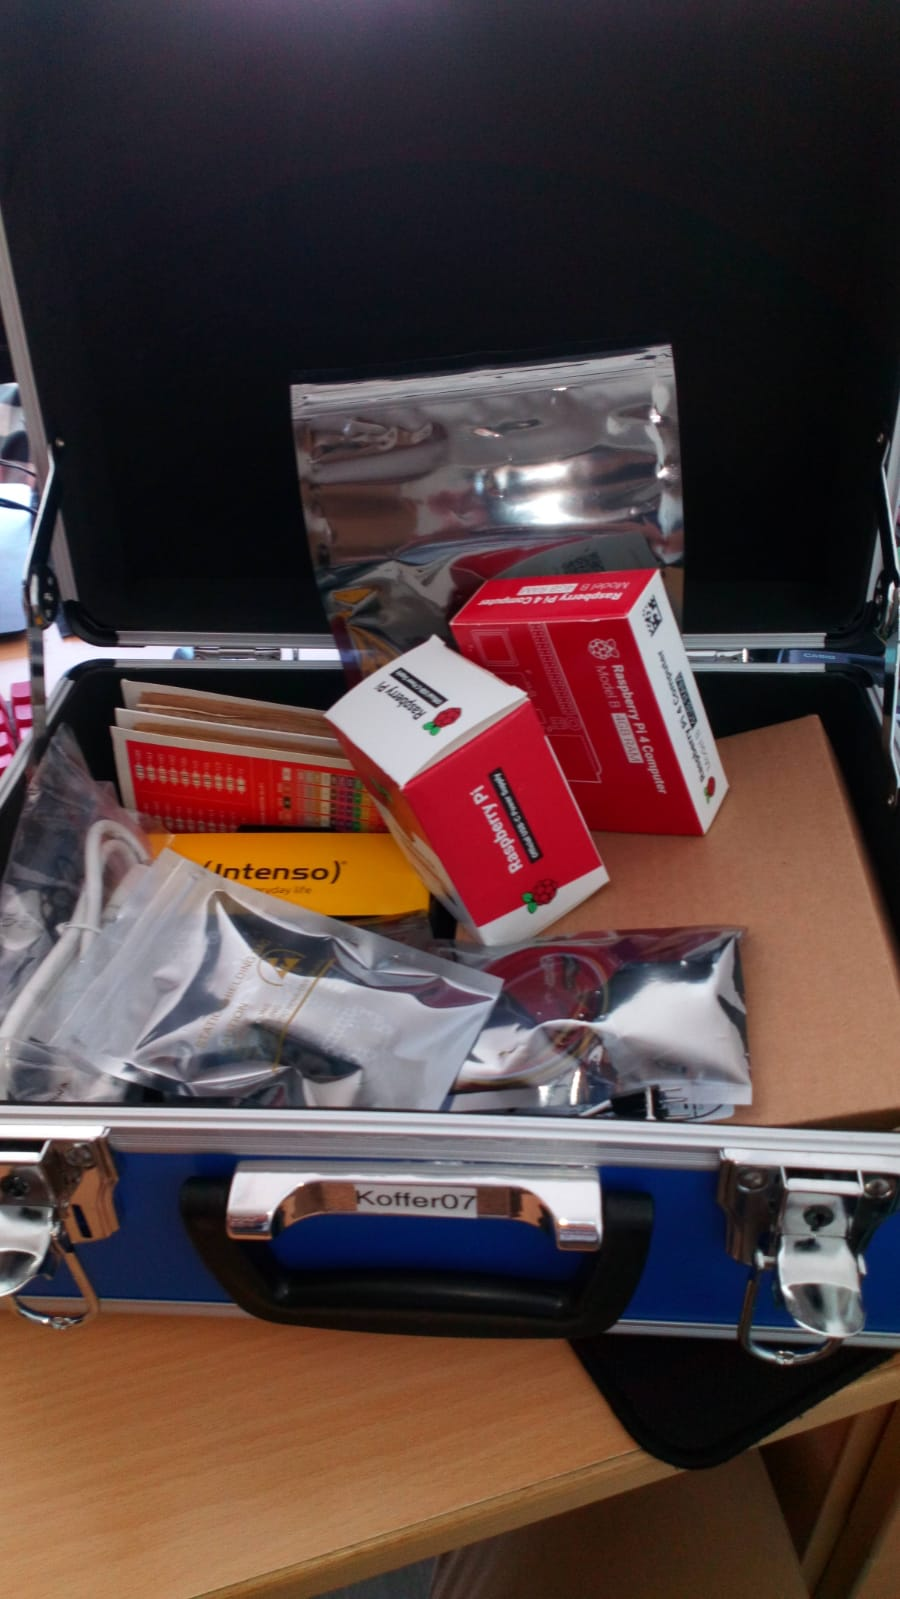
\includegraphics[width=\linewidth]{lernportfolio_assets/Buggy_Koffer.jpeg}
    \caption{Der Buggy vor dem Aufbau.}
  \end{subfigure}
  \begin{subfigure}{0.45\linewidth}
    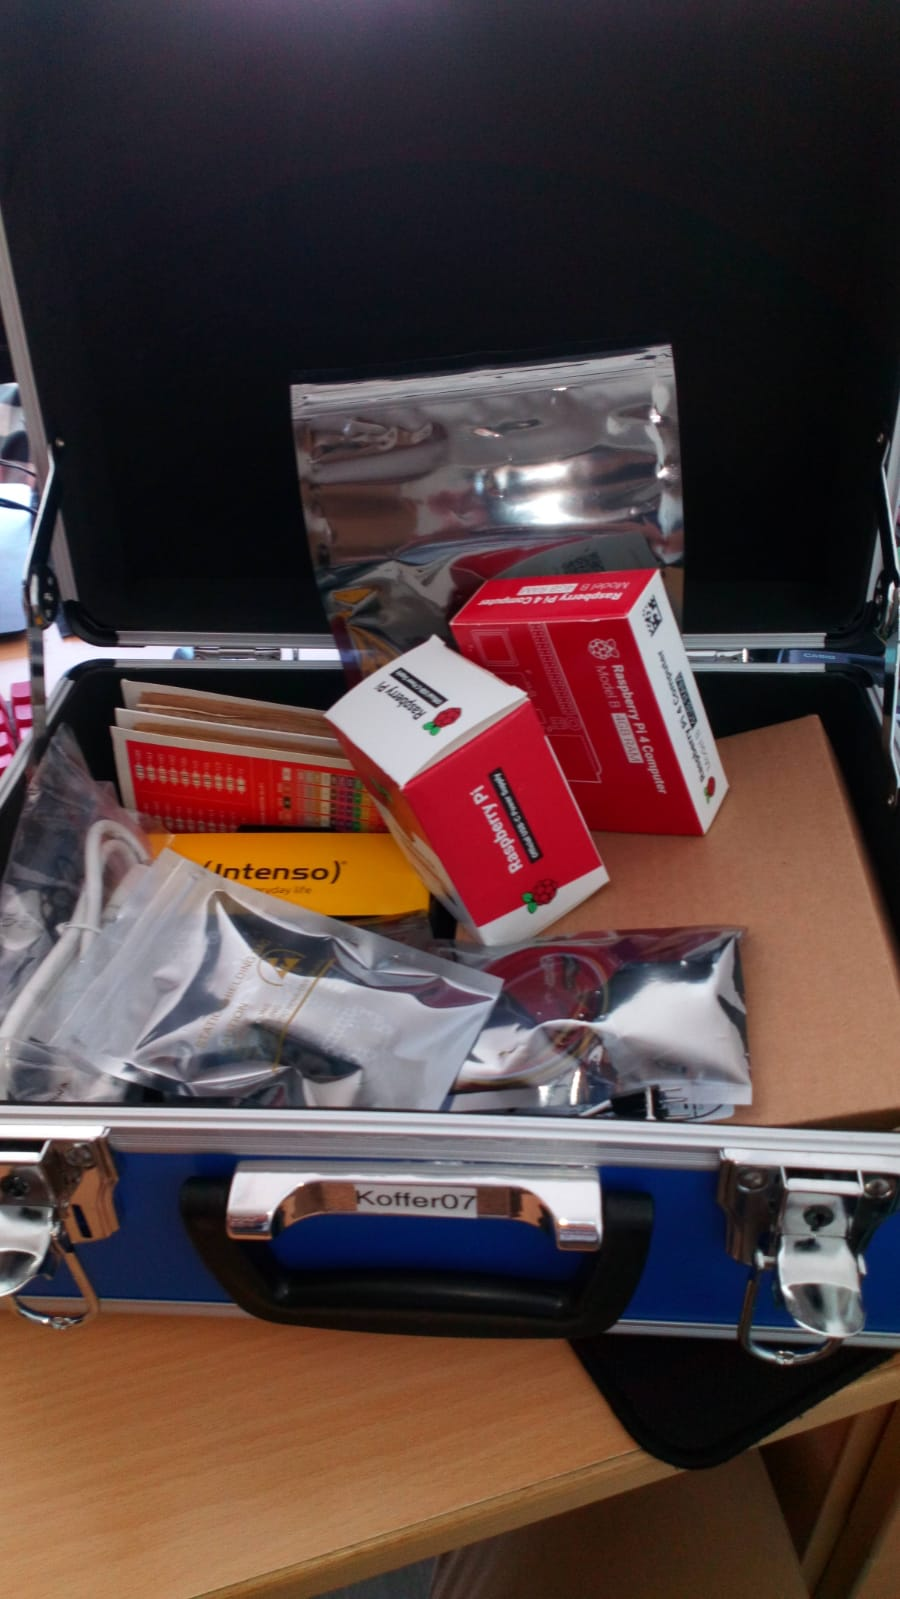
\includegraphics[width=\linewidth]{lernportfolio_assets/Buggy_Koffer.jpeg}
    \caption{Und danach.}
  \end{subfigure}
\end{figure}

Der Buggy wurde vor der Herausgabe des Arbeitsauftrages zusammengebaut. Zwischenschritte sind daher nicht bildlich festgehalten. 

Der Zusammenbau des Buggies verlief problemlos. Der Text ist insgesamt verständlich geschrieben und war eine große Unterstützung.

% Wollen wir das aufnehmen?
% Im Text ist der Genetiv von ``der Buggy'' durchgehend ``des Buggies''. Mit Verweis
% auf \url{https://www.duden.de/rechtschreibung/Buggy} ist der korrekte - und
% kontraintuitive - Genetiv ``des Buggys''.
In den meisten Bildern (außer auf Seite IV) ist der Buggy mit roter Platte gezeigt, wenngleich die Anleitung hier den weißen Winkel vorsieht. Eine Anmerkung, dass der Buggy im Folgendem mit roter Platte statt Winkel gezeigt wird, hätte eine kurze Verwirrung meinerseits verhindert.

Als Ubuntu-Nutzer muss man keine zusätzliche Software installieren um eine SSH-Verbindung herzustellen. Eine Ergänzung, dass \href{https://invisible-island.net/xterm/}{XTerm} eine Empfehlung an die Windows-Nutzer ist, wäre daher angebracht. Bei dieser Bemerkung wird davon ausgegangen, dass mit XTerm an dieser Stelle \href{https://mobaxterm.mobatek.net/}{MobaXterm} gemeint ist und nicht der Terminal Emulator XTerm. 

Für den kompletten Zusammenbau wurden insgesamt 1 Stunden benötigt. Die meiste Zeit nahm die SSH-Verbindung in Anspruch.

% TODO 1.4

\end{document}
